%%%%%%%%%%%%%%%%%%%%%%%%%%%%%%%%%%%%%%%%%%%%%%%%%%%%%%%%%%%%%%%%%%%%%%%%%%%%%%%%
%%
%%   BornAgain User Manual
%%
%%   homepage:   http://www.bornagainproject.org
%%
%%   copyright:  Forschungszentrum Jülich GmbH 2015
%%
%%   license:    Creative Commons CC-BY-SA
%%
%%   authors:    Scientific Computing Group at MLZ Garching
%%               C. Durniak, M. Ganeva, G. Pospelov, W. Van Herck, J. Wuttke
%%
%%%%%%%%%%%%%%%%%%%%%%%%%%%%%%%%%%%%%%%%%%%%%%%%%%%%%%%%%%%%%%%%%%%%%%%%%%%%%%%%

\def\PyImport#1{%
\lstinputlisting[language=python,style=eclipseboxed,name=ex1,nolol]{../../Examples/python/#1}}

\newpage
\chapter{Using the Python API}  \label{sec:Usage}

\Work{This section is a collection of material that is waiting for revision and
tighter integration with the remaining manual.
Much more detailed instruction on using the Python API can be found in the online Tutorial.}

%%%%%%%%%%%%%%%%%%%%%%%%%%%%%%%%%%%%%%%%%%%%%%%%%%%%%%%%%%%%%%%%%%%%%%%%%%%%%%%%
\section{Running a simulation}
%%%%%%%%%%%%%%%%%%%%%%%%%%%%%%%%%%%%%%%%%%%%%%%%%%%%%%%%%%%%%%%%%%%%%%%%%%%%%%%%

A simulation of GISAS using \BornAgain\ consists of the following steps:
\begin{itemize}
\item define materials by specifying name and refractive index,
\item define layers by specifying thickness, roughness, material,
\item define embedded particles by specifying shape, size,
   constituting material, interference function,
\item embed the particles in layers, specifying density, position, orientation,
\item assemble a multilayered sample,
\item specify input beam and detector characteristics,
\item run the simulation,
\item save the simulated detector image.
\end{itemize}

\noindent
All these steps can be organized in either a Graphical User Interface (GUI) or by providing a Python script with the simulation description.
In the following, we describe how to write a
\Code{Python} script which runs a \BornAgain\ simulation. For tutorials about this programming language, the users are referred to \cite{Lut09}.


% More information about the general software architecture and \BornAgain\ internal design are given in \cref{sec:SoftwareArchitecture}.


%===============================================================================
\subsection{Units:}
%===============================================================================
\index{Units}

By default the angles are expressed in radians and the lengths are given in
nanometers.  But it is possible to use other units by
specifying them right after the value of the corresponding
parameter like, for example, \Code{20.0*micrometer}.


%===============================================================================
\subsection{A first example} \label{sec:Example1Python}
%===============================================================================

In this example, we simulate the scattering from a mixture of
cylindrical and prismatic nanoparticles without any interference
between them. These particles are placed in air, on top
of a substrate.\\ We are going to go through each step of the
simulation. The Python code snippet specific to each stage will be given at
the beginning of the description.
More examples can be found at our project web site \url{http://www.bornagainproject.org/documentation/python_examples}

% But for the sake of completeness the full code is given
% in \cref{PythonSimulationExampleScript}.

%-------------------------------------------------------------------------------
\subsubsection{Importing Python modules}
%-------------------------------------------------------------------------------

\setPyNum
\begin{lstlisting}
import numpy @\label{import_lib_beg}@
import matplotlib
import pylab @\label{import_lib_end}@
from bornagain import * @\label{import_ba}@
\end{lstlisting}
We start by importing different functions from external
modules, for example \Code{NumPy} (lines~\ref{import_lib_beg}-\ref{import_lib_end}), which
is a fundamental package for scientific computing with Python
\cite{s:numpy}.  In particular, line~\ref{import_ba}
imports the features of \BornAgain\ software.

%-------------------------------------------------------------------------------
\subsubsection{Defining the materials}
%-------------------------------------------------------------------------------

\begin{lstlisting}
def get_sample(): @\label{def_function}@
    """
    Build and return the sample representing cylinders and pyramids on top of substrate without interference.
   """
    # defining materials @\label{material1}@
    m_air = HomogeneousMaterial("Air", 0.0, 0.0)  @\label{material2}@
    m_substrate = HomogeneousMaterial("Substrate", 6e-6, 2e-8) @\label{material3}@
    m_particle = HomogeneousMaterial("Particle", 6e-4, 2e-8) @\label{materialparticle}@

\end{lstlisting}
Line~\ref{def_function} marks the beginning of the
function to define our sample. Lines~\ref{material2}, \ref{material3} and \ref{materialparticle} define different
materials using class \Code{HomogeneousMaterial}. The general syntax is the following
\setPy
\begin{lstlisting}
<material_name> = HomogeneousMaterial("name", delta, beta)
\end{lstlisting}
where \Code{name} is the name of the
material associated with its complex refractive index
n=1-\Code{delta} +i \Code{beta}. \Code{<material\_name>} is later used when
referring to this particular material. The three materials defined in this example are \Code{Air} with a refractive
index of 1 (\Code{delta = beta = 0}), a \Code{Substrate} associated with a complex refractive index
equal to $1-6\times 10^{-6} +i2\times 10^{-8} $, and the material of the particles, whose refractive index is \Code{n}$=1-6\times 10^{-4}+i2\times 10^{-8}$.

%-------------------------------------------------------------------------------
\subsubsection{Defining the particles}
%-------------------------------------------------------------------------------
\setPyNum
\begin{lstlisting}
    # collection of particles @\label{particles1}@
    cylinder_ff = FormFactorCylinder(5*nanometer, 5*nanometer) @\label{particlescyl1}@
    cylinder = Particle(m_particle, cylinder_ff) @\label{particlescyl2}@
    prism_ff = FormFactorPrism3(10*nanometer, 5*nanometer) @\label{particlesprism1}@
    prism = Particle(m_particle, prism_ff) @\label{particlesprism2}@
\end{lstlisting}
We implement two different shapes of particles: cylinders and
prisms (\idest  elongated particles with a constant equilateral triangular cross section).

All particles implemented in \BornAgain\ are defined by their
form factors (see \cref{SPFF}), their sizes and the material
they are made of. Here, for the
cylindrical particle, we input its radius and height.  For the prism,
the possible inputs are the length of one side of its equilateral triangular
base and its height.

In order to define a particle, we proceed in two steps. For example for
the cylindrical particle, we first specify the form factor of a cylinder with
its radius and height, both equal to 5 nanometers in this particular
case (see line~\ref{particlescyl1}). Then we associate this shape with
the constituting material as in line~\ref{particlescyl2}.
The same procedure has been applied for the prism in lines~\ref{particlesprism1} and \ref{particlesprism2}, respectively.

%-------------------------------------------------------------------------------
\subsubsection{Characterizing particles assembly}
%-------------------------------------------------------------------------------
\begin{lstlisting}
    particle_layout = ParticleLayout()  @\label{particlesdecor1}@
    particle_layout.addParticle(cylinder, 0.5)  @\label{particlesdecor2}@
    particle_layout.addParticle(prism, 0.5)@\label{particlesdecor3}@
    interference = InterferenceFunctionNone()  @\label{particlesnointerf}@
    particle_layout.addInterferenceFunction(interference)  @\label{particlesinterf}@
\end{lstlisting}
The object which holds the information about the positions and densities of particles
in our sample is called \Code{ParticleLayout}
(line~\ref{particlesdecor1}). We use the associated function \Code{addParticle}
for each particle shape (lines~\ref{particlesdecor2}, \ref{particlesdecor3}). Its general syntax is
\setPy
\begin{lstlisting}
addParticle(<particle_name>, abundance)
\end{lstlisting}
where \Code{<particle\_name>} is the name used to define the particles
(lines~\ref{particlescyl2} and \ref{particlesprism2}) and
\Code{abundance} is the proportion of this type of particles,
normalized to the total number of particles. Here we have 50\% of cylinders
and 50\% of prisms.
Lines~\ref{particlesnointerf} and
\ref{particlesinterf} specify that there is \textbf{no coherent interference} between
the waves scattered by these particles.
In this case, the intensity is given by the incoherent sum~\cref{EIdInc}.

%-------------------------------------------------------------------------------
\subsubsection{Multilayer}
%-------------------------------------------------------------------------------
\setPyNum
\begin{lstlisting}
# air layer with particles and substrate form multi layer  @\label{sampleassembling}@
    air_layer = Layer(m_air) @\label{airlayer}@
    air_layer.addLayout(particle_layout) @\label{airlayerdecorator}@
    substrate_layer = Layer(m_substrate, 0)  @\label{substratelayer}@
    multi_layer = MultiLayer() @\label{multilayercanvas}@
    multi_layer.addLayer(air_layer) @\label{layerairdecor}@
    multi_layer.addLayer(substrate_layer) @\label{layersubstrate}@
    return multi_layer @\label{returnmlayer}@
\end{lstlisting}
We now have to configure our sample. For this first example,
the particles, \idest  cylinders and prisms, are on top of a substrate in an
air layer. \textbf{The order in which we define these layers is important: we
start from the top layer down to the bottom one}.

Let us start with the air layer. It contains the particles. In
line~\ref{airlayer}, we use the previously defined \Code{m\_air}
(="air" material) (line~\ref{material2}). The command in line~\ref{airlayerdecorator} shows that this layer contains particles
which are defined using particle layout object. The substrate layer
only contains the substrate material (line~\ref{substratelayer}).
%Note that the
%\Code{depth} is referenced to the bottom of the top layer (negative
%values would correspond to particles floating above layer 1 as
%the vertical axis is pointing upwards).

There are different possible syntaxes to define a layer. As shown in
lines~\ref{airlayer} and \ref{substratelayer}, we can use
\Code{Layer(<material\_name>,thickness)} or
\Code{Layer(<material\_name>)}. The second case corresponds
to the default value of the \Code{thickness}, equal to 0. The \Code{thickness} is
expressed in  nanometers.

Our two layers are now fully characterized. The sample is assembled using
\Code{MultiLayer()} constructor (line~\ref{multilayercanvas}): we start with the air layer decorated
with the particles (line~\ref{layerairdecor}), which is the layer at
the top and end with the bottom layer, which is the
substrate (line~\ref{layersubstrate}).

%-------------------------------------------------------------------------------
\subsubsection{Characterizing the input beam and output detector}
%-------------------------------------------------------------------------------

\begin{lstlisting}
def get_simulation():  @\label{run1}@
    """
    Create and return GISAXS simulation with beam and detector defined
    """
    simulation = Simulation() @\label{run2}@
    simulation.setDetectorParameters(100, -1.0*degree, 1.0*degree, 100, 0.0*degree, 2.0*degree) @\label{rundetector}@
    simulation.setBeamParameters(1.0*angstrom, 0.2*degree, 0.0*degree) @\label{runbeam}@
    return simulation @\label{returnsimul}@
\end{lstlisting}
Line~\ref{run2} creates a \Code{Simulation()} object.
Line~\ref{rundetector} sets the histogram bins of the default spherical detector (\cref{SRefDet}).
Line~\ref{runbeam} defines the incoming beam (\cref{SRefBeam}).


%-------------------------------------------------------------------------------
\subsubsection{Running the simulation and plotting the results}
%-------------------------------------------------------------------------------

\begin{lstlisting}
def run_simulation(): @\label{run_simulation}@
    """
   Run simulation and plot results
    """
    sample = get_sample() @\label{get_sample}@
    simulation = get_simulation() @\label{get_simulation}@
    simulation.setSample(sample)  @\label{setsample}@
    simulation.runSimulation()  @\label{runsimul}@
    result = simulation.getIntensityData().getArray() + 1  # for log scale  @\label{outputdata}@
    pylab.imshow(numpy.rot90(result, 1), norm=matplotlib.colors.LogNorm(), extent=[-1.0, 1.0, 0, 2.0]) @\label{plot1}@
    pylab.show() @\label{plot2}@
\end{lstlisting}
%In function \Code{run\_simulation()}, we associate the sample
%characterised by function \Code{get\_sample()} with the input beam and
%output detector, defined in function \Code{get\_simulation()} (line~\ref{runsample}).
The function, whose definition starts from line~\ref{run_simulation}, gathers all
items. We create the sample and the simulation objects at the lines
~\ref{get_sample} and \ref{get_simulation}, using calls to the previously defined functions. We assign the sample to the simulation at line ~\ref{setsample} and
finally launch the simulation at line ~\ref{runsimul}.

In line~\ref{outputdata} we obtain the simulated intensity
as a function of outgoing angles $\alpha_f$ and $\phi_f$ for further
uses (plots, fits,\ldots) as a \Code{NumPy} array containing
\Code{n\_phi}$\times$\Code{n\_alpha}
datapoints. Lines~\ref{plot1}-\ref{plot2} produces the two-dimensional
contour plot of the intensity as a function of $\alpha_f$ and
$\phi_f$ shown in \cref{fig:output_ex1}.

\begin{figure}[htbp]
  \begin{center}
   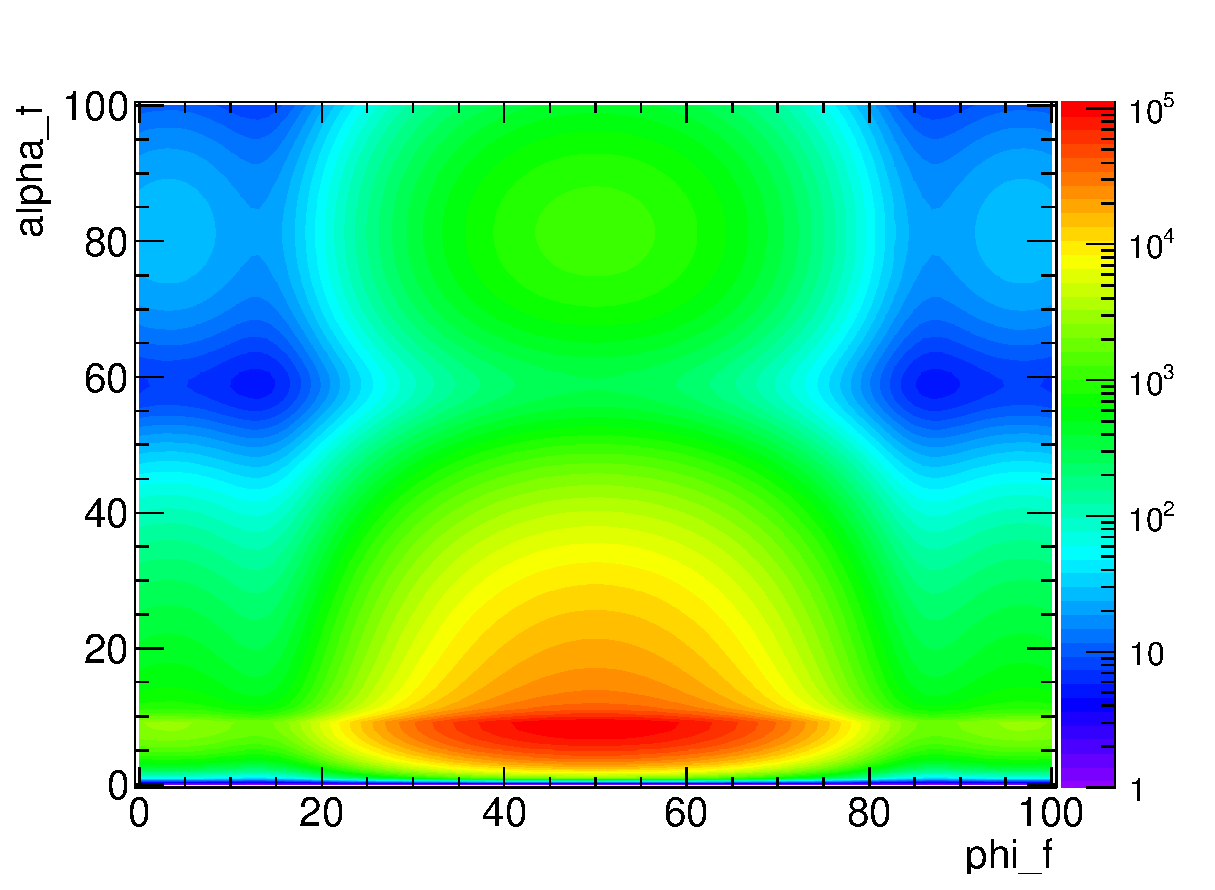
\includegraphics[clip=true, width=120mm]{fig/gisasmap/Manual_ex1.eps}
  \end{center}
  \caption[Example 1: Simulated grazing-incidence small-angle X-ray scattering from a mixture of
cylindrical and prismatic nanoparticles without any interference, deposited on top
of a substrate]{Simulated grazing-incidence small-angle X-ray scattering from a mixture of
cylindrical and prismatic nanoparticles without any interference, deposited on top
of a substrate. The input beam is characterized by a wavelength
$\lambda$ of 1~\AA\ and incident angles $\alpha_i=0.2^{\circ}$, $\phi_i=0^{\circ}$. The
cylinders have a radius and a height both equal to 5~nm, the prisms
are characterized by a side length equal to 10~nm and they are 5~nm high. The
material of the particles has a refractive index of $1-6\times 10^{-4}+i2\times 10^{-8}$. For the substrate
it is equal to $1-6\times 10^{-6} +i2\times 10^{-8} $. The color scale
is associated with the output intensity in arbitrary units. }
\label{fig:output_ex1}
\end{figure}


%===============================================================================
\subsection{Working with sample parameters}
   \label{sec:WorkingWithSampleParameters}
%===============================================================================


This section gives additional details about the manipulation of sample parameters
during run time; that is after the sample has already been constructed.
For a single simulation this is normally not necessary. However it might be useful
during interactive work when the user tries to find optimal sample parameters by
running a series of simulations.
A similar task also arises when the theoretical model, composed of the
description of the sample and of the simulation, is used for fitting real data.
In this case, the fitting kernel requires a list of the existing sample parameters
and a mechanism for changing the values of these parameters in order to find
their optima.

In \BornAgain\ this is done using the so-called sample parameter pool
mechanism. We are going to briefly explain this approach using the example
of \cref{sec:Example1Python}.

In \BornAgain\ a sample is described by a hierarchical tree of objects.
For the multilayer created in the previous section this tree can be graphically
represented as shown in \cref{fig:sample_tree}. Similar trees can
be printed in a Python
session by running \Code{multi\_layer.printSampleTree()}

\begin{figure}[p!]

\tikzstyle{every node}=[draw=black,thick,anchor=west]
\tikzstyle{selected}=[draw=red,fill=red!30]
\tikzstyle{optional}=[dashed,fill=gray!50]
\begin{tikzpicture}[%
  grow via three points={one child at (0.5,-0.7) and
  two children at (0.5,-0.7) and (0.5,-1.4)},
  edge from parent path={(\tikzparentnode.south) |- (\tikzchildnode.west)}]
  \node {MultiLayer}
    child { node {Layer \#0}
		child { node {ParticleLayout }
			child { node {Particle Info 0}
				child {node {Particle }
					child { node {FormFactorCylinder}
						child { node [optional] { radius:5.0} }
						child { node [optional] { height:5.0} }
					}
				}
    			child [missing] {}
    			child [missing] {}
			    child [missing] {}
				child {node [optional] { abundance:0.5} }
				child {node [optional] { depth:0.0} }
			}
    		child [missing] {}
    		child [missing] {}
			child [missing] {}
    		child [missing] {}
    		child [missing] {}
			child [missing] {}
			child { node {Particle Info 1}
				child {node {Particle }
					child { node {FormFactorPrism3}
						child { node [optional] { length:10.0} }
						child { node [optional] { height:5.0} }
					}
				}
    			child [missing] {}
    			child [missing] {}
			    child [missing] {}
				child {node [optional] { abundance:0.5} }
				child {node [optional] { depth:0.0} }
			}
		}
		child [missing] {}
   		child [missing] {}
	    child [missing] {}
		child [missing] {}
   		child [missing] {}
	    child [missing] {}
	    child [missing] {}
		child [missing] {}
   		child [missing] {}
	    child [missing] {}
		child [missing] {}
   		child [missing] {}
	    child [missing] {}
	    child [missing] {}
		child {node [optional] { thickness:0.0} }
    }
	child [missing] {}
   	child [missing] {}
	child [missing] {}
   	child [missing] {}
	child [missing] {}
	child [missing] {}
   	child [missing] {}
	child [missing] {}
   	child [missing] {}
	child [missing] {}
	child [missing] {}
   	child [missing] {}
	child [missing] {}
   	child [missing] {}
	child [missing] {}
	child [missing] {}
	child { node {Layer interface \#0}
    	child {node { roughness}
    		child {node [optional] { corrlength:0.0} }
    		child {node [optional] { hurst:0.0} }
    		child {node [optional] { sigma:0.0} }
    	}
	}
   	child [missing] {}
	child [missing] {}
	child [missing] {}
    child { node {Layer \#1}
    	child {node [optional] { thickness:0.0} }
    }
	child [missing] {}
    child { node [optional] {CrossCorrLength:0.0} };

\end{tikzpicture}
\caption{Tree representation of the sample structure.}
\label{fig:sample_tree}
\end{figure}


The top \Code{MultiLayer} object is composed of three children, namely
\Code{Layer \#0, Layer Interface \#0} and \Code{Layer \#1}. The
children objects might themselves also be decomposed into tree-like structures. For example,
\Code{Layer \#0} contains a \Code{ParticleLayout} object, which holds information
related to the two types of particles populating the layer. All numerical values used
during the sample construction (thickness of layers, size of particles, roughness parameters) are part of the same tree structure.
They are marked in the figure with shaded gray boxes.

These values are registered in the sample parameter pool using the name
composed of the corresponding nodes' names. And they can be accessed/changed
during run time. For example, the \Code{height} of the cylinders
populating the first layer can be changed from the
current value of $5~\rm{nm}$ to $1~\rm{nm}$ by running the command

\begin{lstlisting}[language=shell, style=commandline]
multi_layer.setParameterValue('/MultiLayer/Layer0/ParticleLayout/ParticleInfo0/Particle/FormFactorCylinder/height', 1.0)
\end{lstlisting}


A list of the names and values of all registered sample's parameters
can be displayed using the command

\begin{lstlisting}[language=shell, style=commandline]
> multi_layer.printParameters()
The sample contains following parameters ('name':value)
'/MultiLayer/Layer0/ParticleLayout/ParticleInfo0/Particle/FormFactorCylinder/height':5
'/MultiLayer/Layer0/ParticleLayout/ParticleInfo0/Particle/FormFactorCylinder/radius':5
'/MultiLayer/Layer0/ParticleLayout/ParticleInfo0/abundance':0.5
'/MultiLayer/Layer0/ParticleLayout/ParticleInfo0/depth':0
'/MultiLayer/Layer0/ParticleLayout/ParticleInfo1/Particle/FormFactorPrism3/length':5
'/MultiLayer/Layer0/ParticleLayout/ParticleInfo1/Particle/FormFactorPrism3/height':5
'/MultiLayer/Layer0/ParticleLayout/ParticleInfo1/abundance':0.5
'/MultiLayer/Layer0/ParticleLayout/ParticleInfo1/depth':0
'/MultiLayer/Layer0/thickness':0
'/MultiLayer/Layer1/thickness':0
'/MultiLayer/LayerInterface/roughness/corrlength':0
'/MultiLayer/LayerInterface/roughness/hurst':0
'/MultiLayer/LayerInterface/roughness/sigma':0
'/MultiLayer/crossCorrLength':0
\end{lstlisting}

Wildcards \Code{'*'} can be used to reduce typing or to work on a group
of parameters. In the example below, the first command will change the
height of all cylinders in the same way, as in the previous example. The second line will change simultaneously the height of {\it both} cylinders and prisms.
\begin{lstlisting}[language=shell, style=commandline]
multi_layer.setParameterValue('*FormFactorCylinder/height', 1.0)
multi_layer.setParameterValue('*height', 1.0)
\end{lstlisting}

The complete example described in this section can be found at
\begin{lstlisting}[language=shell, style=commandline]
./Examples/python/fitting/ex001_SampleParametersIntro/SampleParametersIntro.py
\end{lstlisting}
